\documentclass[10pt,a4paper]{article}

\usepackage[italian]{babel}
\usepackage[usenames,dvipsnames,table]{xcolor}
\usepackage[utf8]{inputenc}
\usepackage[T1]{fontenc}
\usepackage{soul}
\usepackage[a4paper, portrait, margin=2.5cm]{geometry}
\usepackage{array}
\usepackage{tabularx} 
\usepackage{booktabs}
\usepackage{multicol}
\usepackage{amsmath}
\usepackage{amsfonts}
\usepackage{amssymb}
\usepackage{algorithmicx}
\usepackage[noend]{algpseudocode}
\usepackage{wrapfig}
\usepackage{graphicx}
\usepackage{hyperref}

\graphicspath{ {./images/} }

\begin{document}

\title{Data Flow Analysis \\
\large Assignment 2}
\author{Iacopo Ruzzier, Daniele Fassetta, Anna Semeraro}

\maketitle
\tableofcontents

\newpage

\section{Introduzione}

Paragrafo introduttivo

\section{Very Busy Expressions}
\subsection{Definizione del problema}

Definizione a parole di Gen, ...


\begin{table}[h!]
  \centering
  \begin{tabular}{|l|p{4cm}|}
    \hline
    \textbf{} & \textbf{Very Busy Expressions} \\
    \hline
    Domain & Espressioni\\
    \hline
    Direction & backward\\
    \hline
    Transfer function & $f_b = Gen_b \cup (x - Kill_b) $\\
    \hline
    Meet Operation ($\land$) & $\cap$ \\
    \hline
    Boundary Condition & $in[exit] = \emptyset$ \\
    \hline
    Initial interior points & $in[b] = \mathcal{U}$ \\
    \hline
  \end{tabular}
  \caption{Very busy expressions}
\end{table}

\subsection{Esempio}

\begin{figure}[h]
  \centering
  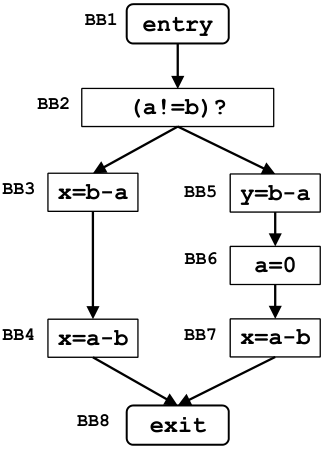
\includegraphics[width=.5\textwidth]{example-1.png}
  \caption{Esempio 1}
\end{figure}

\begin{table}[h!]
\centering
\renewcommand{\arraystretch}{1.5}
\rowcolors{2}{gray!10}{white}
\begin{tabular}{|c|c|c|c|c|c|c|}
\hline
\rowcolor{blue!30}
 & \multicolumn{2}{c|}{Iterazione 1} & \multicolumn{2}{c|}{Iterazione 2} & \multicolumn{2}{c|}{Iterazione 3} \\
\rowcolor{blue!30}
 & IN[B] & OUT[B] & IN[B] & OUT[B] & IN[B] & OUT[B] \\
\hline
BB1 & $\langle \ldots \rangle$ & $\langle \ldots \rangle$ & & & & \\
\hline
BB2 & & & & & & \\
\hline
BB3 & & & & & & \\
\hline
\end{tabular}
\end{table}




\section{Dominator Analysis}
\subsection{Definizione del problema}
\begin{table}[h!]
  \centering
  \begin{tabular}{|l|p{4cm}|}
    \hline
    \textbf{} & \textbf{Donator Analysis} \\
    \hline
    Domain & Basic blocks\\
    \hline
    Direction & forward\\
    \hline
    Transfer function & $f_b = Gen_b \cup Kill_b$\\
    \hline
    Meet Operation (\(\land\)) & $\cap$ \\
    \hline
    Boundary Condition & $in[entry] = \emptyset $\\
    \hline
    Initial interior points & $in[b] = \emptyset $ \\
    \hline
  \end{tabular}
  \caption{Dominator analysis}
\end{table}

\subsection{Esempio}
\begin{figure}[h]
  \centering
  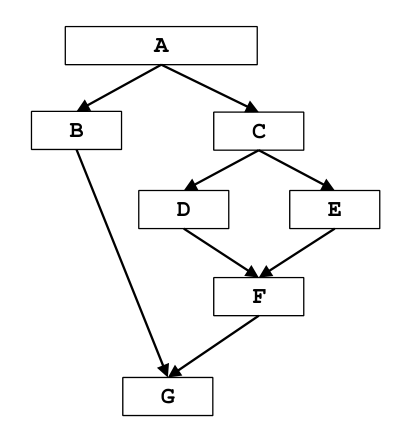
\includegraphics[width=.5\textwidth]{example-2.png}
  \caption{Esempio 2}
\end{figure}
\begin{table}[h!]
\centering
\renewcommand{\arraystretch}{1.5}
\rowcolors{2}{gray!10}{white}
\begin{tabular}{|c|c|c|c|c|c|c|}
\hline
\rowcolor{blue!30}
 & \multicolumn{2}{c|}{Iterazione 1} & \multicolumn{2}{c|}{Iterazione 2} & \multicolumn{2}{c|}{Iterazione 3} \\
\rowcolor{blue!30}
 & IN[B] & OUT[B] & IN[B] & OUT[B] & IN[B] & OUT[B] \\
\hline
BB1 & $\langle \ldots \rangle$ & $\langle \ldots \rangle$ & & & & \\
\hline
BB2 & & & & & & \\
\hline
BB3 & & & & & & \\
\hline
\end{tabular}
\end{table}


\section{Constant propagation}

\subsection{Definzione del problema}

\begin{table}[h!]
  \centering
  \begin{tabular}{|l|p{4cm}|}
    \hline
    \textbf{} & \textbf{Constant Propagation} \\
    \hline
    Domain & coppie (variabile, valore)\\
    \hline
    Direction & forward \\
    \hline
    Transfer function &  \\
    \hline
    Meet Operation (\(\land\)) & \\
    \hline
    Boundary Condition & \\
    \hline
    Initial interior points & \\
    \hline
  \end{tabular}
  \caption{Constant propagation}
\end{table}

\subsection{Esempio}

\begin{figure}[h]
  \centering
  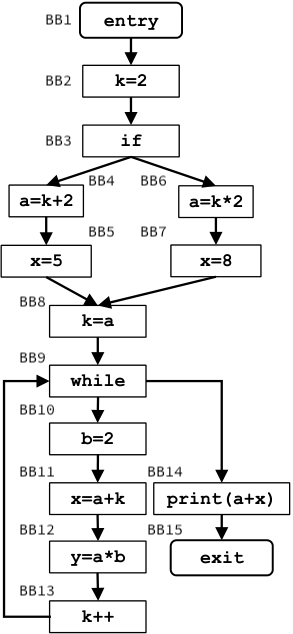
\includegraphics[width=.5\textwidth]{example-3.png}
  \caption{Esempio 3}
\end{figure}

\begin{table}[h!]
\centering
\renewcommand{\arraystretch}{1.5}
\rowcolors{2}{gray!10}{white}
\begin{tabular}{|c|c|c|c|c|c|c|}
\hline
\rowcolor{blue!30}
 & \multicolumn{2}{c|}{Iterazione 1} & \multicolumn{2}{c|}{Iterazione 2} & \multicolumn{2}{c|}{Iterazione 3} \\
\rowcolor{blue!30}
 & IN[B] & OUT[B] & IN[B] & OUT[B] & IN[B] & OUT[B] \\
\hline
BB1 & $\langle \ldots \rangle$ & $\langle \ldots \rangle$ & & & & \\
\hline
BB2 & & & & & & \\
\hline
BB3 & & & & & & \\
\hline
\end{tabular}
\end{table}

\end{document}
